\documentclass[12pt]{article}
\usepackage[english]{babel}
\usepackage{natbib}
\usepackage{url}
\usepackage[utf8x]{inputenc}
\usepackage{amsmath}
\usepackage{textcomp}
\usepackage{enumitem}
\usepackage{graphicx}
\usepackage{listings}
\usepackage{xcolor}
\graphicspath{{images/}}
\usepackage{parskip}
\usepackage{hyperref}
\usepackage{fancyhdr}
\usepackage{vmargin}
\setmarginsrb{3 cm}{2.5 cm}{3 cm}{2.5 cm}{1 cm}{1.5 cm}{1 cm}{1.5 cm}
\setlength{\parindent}{5ex}
							

\lstdefinestyle{DOS}
{
    backgroundcolor=\color{black},
    basicstyle=\scriptsize\color{white}\ttfamily
}

\makeatletter
\let\thetitle\@title

\let\thedate\@date
\makeatother

\pagestyle{fancy}
\fancyhf{}
\rhead{\theauthor}
\lhead{\thetitle}
\cfoot{\thepage}

\begin{document}

%%%%%%%%%%%%%%%%%%%%%%%%%%%%%%%%%%%%%%%%%%%%%%%%%%%%%%%%%%%%%%%%%%%%%%%%%%%%%%%%%%%%%%%%%

\begin{titlepage}
	\centering
   % \vspace*{0.5 cm}
    
\includegraphics[scale = 0.35]{iiitm.jpg}\\[1.0 cm]	% University Logo
    \textsc{\large Atal Bihari Vajpayee - Indian Institute Of } \\[0.5cm]
    \textsc{\large Information Technology and Management,} \\[0.5cm]
    \textsc{\large Gwalior}\\[2.0 cm]
    \textsc{\large B.Tech Compute Science and Engineering}\\[0.8 cm]

	\textsc{\Large \textbf{Summer Project} }\\[0.5 cm]				% Course Code
	\textsc{\large \textbf{SOURCE CODE PLAGIARISM DETECTION SYSTEM} }\\[1.5 cm]
	\rule[0pt]{\linewidth}{1pt}
	
% 	\begin{minipage}{0.5\textwidth}
    \begin{flushright}
    	\textbf{\large   Divyansh Falodiya}\linebreak
		\textbf{\large  2019BCS-020}\linebreak
	\end{flushright}
	%		\emph{STUDENT ID :} \\
		%	153402341 - Manish Kumar\linebreak		
			
% 	\end{minipage}\\[2 cm]
	
    \begin{flushleft}
	
	\begin{minipage}{0.4\textwidth}
			\emph{Under the supervision of } \\
		\textbf{Dr. Santosh Singh Rathore}\linebreak
	\end{minipage}\\[2 cm]

	\end{flushleft}
 
	\vfill
	
\end{titlepage}

%%%%%%%%%%%%%%%%%%%%%%%%%%%%%%%%%%%%%%%%%%%%%%%%%%%%%%%%%%%%%%%%%%%%%%%%%%%%%%%%%%%%%%%%%

\tableofcontents
\pagebreak
%%%%%%%%%%%%%%%%%%%%%%%%%%%%%%%%%%%%%%%%%%%%%%%%%%%%%%%%%%%%%%%%%%%%%%%%%%%%%%%%%%%%%%%%%

\section{Abstract}
Plagiarism, in its essence, is the representation of other's ideas and thoughts as one's own. In academic context, there are differing definitions of Plagiarism which is rather subjective. Plagiarism is considered to be ethically wrong, be it of any kind. It is considered as a violation of academic integrity and may lead to different kind of penalties. There can be serious consequences to plagiarism :\par
\begin{itemize}
    \item As a student, it can lead to failure in the course or even cancellation of the degree.
    \item As an academic professional, it can lead to some serious legal issues including copyright infringement and can take down the professional's reputation.
\end{itemize}
From an academic perspective, plagiarism of source code files is considered as a form of academic dishonesty. Students usually try to submit assignments by copying from their peers or from the internet. Detecting plagiarism in source code files manually is often time consuming as there can be a lot of files involved.\par
This project aims at providing a solution to the 'Plague of Plagiarism' in the academic world so as to detect plagiarism among source code files.

\pagebreak

\section{Introduction}
\subsection{Plagiarism}
Plagiarism, as we know, is the act of imitating or copying someone else's work and presenting it as your own. It is very common in the academic environment where students usually copy assignments from their peers, modify it to conceal the fact that it is plagiarised and submit it as their own work. This can make it difficult for the instructor to identify plagiarised assignments manually. \par
From the perspective of academic professionals, there is no commonly agreed definition of what constitutes a source code plagiarism. For instance, the problem statement may require the use of a common algorithm, so every submission will have the same algorithm. So, surely the assignments will be similar but nothing can be said about it being plagiarised. \par

\subsection{Background}
A lot of research has been put into the field of source code plagiarism and a ton of tools have been developed that work quite well. One of the earliest tools developed was Plague. It converts the code into structure files and compares them using Heckel algorithm and it only supports C language. Another such tool is MOSS which uses a string matching algorithm to divide the code into n-grams, hash them and create fingerprints of the hashes using Winnowing algorithm and compare these fingerprints. Not only Plague and MOSS, but there are quite a handful of other tools as well such as JPlag, YAP, Sherlock, and many more, some of which are open source as well.


\subsection{Motivation}
Plagiarising code assignments constitutes a form of academic deception. Students usually plagiarise due to either laziness or the lack of academic ability. It is important that students try and do these assignments by themselves. Not only in academic institutions, plagiarism of source code is also found on online coding platforms and sometimes, we may even find that an entire software is plagiarised. \par
Plagiarisation of any academic material is considered to be an ethical offense and may lead the person to some serious consequences. In legal terms, it is considered as literary theft. The ethics of plagiarism is the ethics of stealing  \footnote{\url{https://www.plagramme.com/ethics-of-plagiarism}}.

\subsection{Problem Statement}
Detecting plagiarism in source code files, be it two files or a hundred files, is tedious task to do manually for any instructor. With this in mind, the question that comes to mind is "Can plagiarism be detected among different source code files?" or "Is it possible to automate the process of plagiarism detection in source code". This project aims to answer the above mentioned questions.

\subsection{Objective}
One of the major objectives of this project is to provide a reliable solution to the academic institutions to detect plagiarism in the submitted assignments using very less computation power. This project has been developed in the form of a CLI tool which, in general, is considered to be faster and more efficient as compared to other interface tools. \par


\section{Literature Review}
Plagiarising assignments in academic institutions is getting way too normalized now-a-days and in this era of online education, young students tend to get attracted towards plagiarising solutions as it seems to provide them an easy way to get things done. Several methods have been proposed for efficient identification of plagiarism after intensive research. \par \textbf{Deimos} is one of the result of such a research which is described in "Automatic Source Code Plagiarism Detection" by Cynthia Kustanto and Inggriani Liem. It works in the following steps : (a) Tokenization, (b) Comparison of tokens using RKR-GST  algorithm. \par
Another approach described in "An AST-based Code Plagiarism Detection System" by Jingling Zhao, Kunfeng Xia, Yilun Fu, Baojiang Cui makes use of abstract syntax trees to identify the similarity of the syntactic structure of the code. This approach is better suitable for plagiarism detection in repositories or programs that may not require the same algorithm for solutions and so the flow of program may be different. \par
This project, however, is heavily inspired from the thesis "An Approach to Source-Code Plagiarism Detection and Investigation Using Latent Semantic Analysis" by Georgina Cosma, Mike Joy which approaches the problem using information retrieval techniques, specifically Latent Semantic Analysis, so as to find the similarity among different programs.

%\pagebreak

\section{Methodology}
\subsection{Flow Chart}
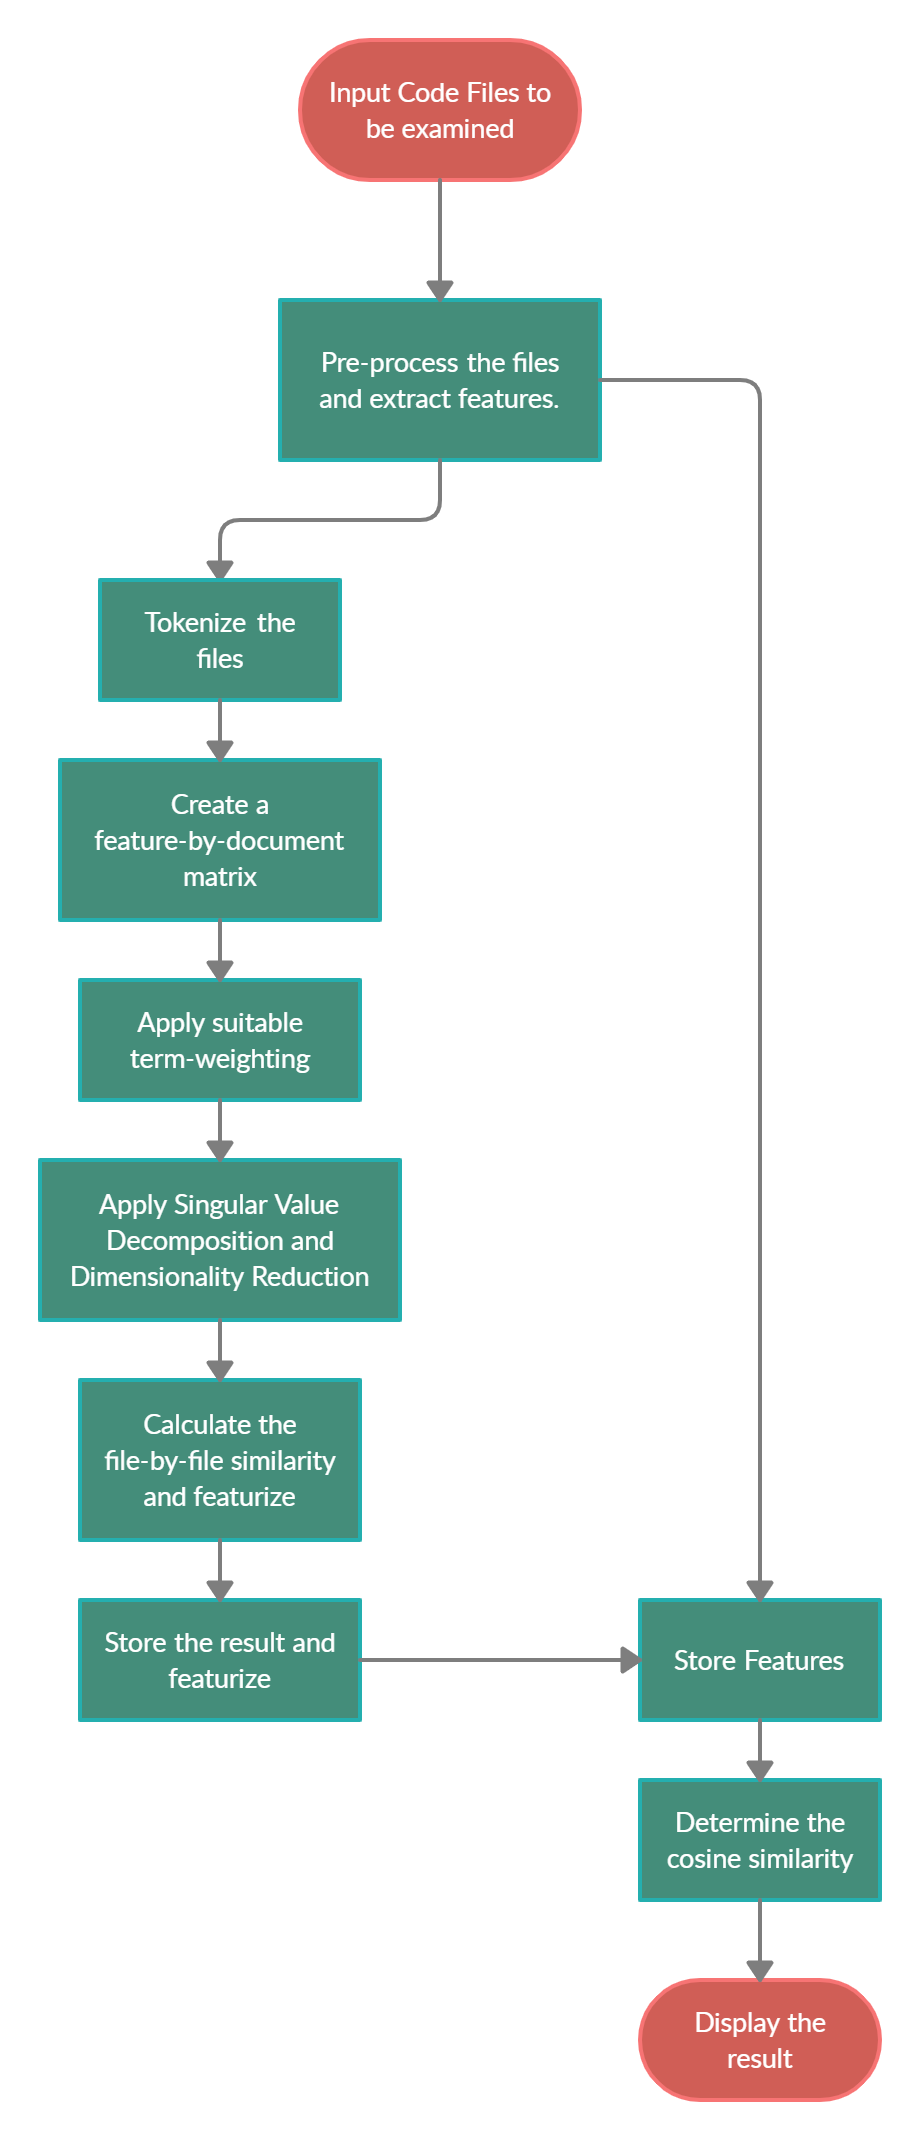
\includegraphics[height=15cm]{flow.png}
\subsection{Implementation}
Based on the fact that this tool needs to be used by instructors for detecting plagiarism, understanding the needs of the instructor is an important part in developing it. It is developed as a python package that works directly from the command line. To install the package on a system, cd into the root of the package\footnote{\url{https://github.com/DivyanshFalodiya/plagiarism-detector}} where setup.py is located and run the following command:
\begin{verbatim}
    >> python setup.py install
\end{verbatim}
This will install the package on the system and add the "plag" command to the PATH variable.
The command to access the tool is "plag".\par
Some examples of the commands are:
\begin{itemize}
    \item Display the version of the tool.
    % \begin{quote}
    \begin{lstlisting}[style=DOS]
    >> plag --version
    \end{lstlisting}
    % \end{quote}
    
    \item Display information about the tool.
    % \begin{quote}
    \begin{lstlisting}[style=DOS]
    >> plag --help
    \end{lstlisting}
    % \end{quote}
    
    \item Sets the process comment argument (-pc) as True and sets the path to the primary file (-p) as "c:/Users/divyansh/data/file1.cpp".
    % \begin{quote}
    \begin{lstlisting}[style=DOS]
    >> plag -pc -p "c:/Users/divyansh/data/file1.cpp"
    \end{lstlisting}
    % \end{quote}
\end{itemize}
There are many more ways to customize the processing other than those described here. \par
It takes two inputs from the user : (a) the primary file that needs to be compared, (b) the folder that contains the files that need to be compared with the primary file. \par
The process that occurs under the hood is as follows:
\begin{enumerate}
    \item All the files input into the system are preprocessed accordingly.
    \begin{itemize}
        \item Features are extracted from the source code such as the number of loops, number of variables, etc.
        \item Comments are removed from the file so that they don't interfere with similarity calculation.
        \item The extracted comments are tokenized if the user intends to.
        \item The source code files are tokenized and any irrelevant tokens are removed.
    \end{itemize}
    \item A term-by-document matrix (TD Matrix) for the tokenized files and the tokenized comments (if required) is created.
    \item The TNC \footnote{TNC Weight = Term Frequency $\times$ Normal Weight of the document} weighting scheme is applied to the code's TD Matrix.
    \item If comments are to be processed, the TF-IDF \footnote{TF-IDF Weight = Term Frequency $\times$ Inverse Document Frequency} weighting scheme is applied to the comment's TD Matrix.
    \item Singular Value Decomposition is applied to the code's TD Matrix and the dimensions of the resultant matrix are reduced suitably. Result = U, $\sigma$, V\textsuperscript{T} (T represents the transpose of the matrix).
    \item The similarity matrix (S) is calculated for the code as well as the comments by (V$\sigma$)(V$\sigma$)\textsuperscript{T}. This matrix is a document-by-document matrix and so, the value $S_{ij}$ represents the similarity between the $i^{th}$ and the $j^{th}$ document.
    \item The features extracted during preprocessing and the similarity value calculated for the code and comments make up another feature vector for the document. Now, the simiarity is calculated using Cosine Similarity.
    \item A detailed report indicating the feature values and the similarity is presented to the user.
\end{enumerate}
%\includegraphics[height=5cm]{download.jpg}

% \section{What awaits in the future?}
% %\section*{i.Arduino Uno}
% The Arduino Uno is a microcontroller board based on the ATmega328. It has 20 digital input/output pins (of which 6 can be used as PWM outputs and 6 can be used as analog inputs), a 16 MHz resonator, a USB connection, a power jack, an in-circuit system programming (ICSP) header, and a reset button.

% %\includegraphics[height=3cm]{ar.jpg}

% %\section*{ii.RF 433MHz Transmitter/Receiver Module}
% These RF modules are very popular among the Arduino tinkerers. The 433MHz transceiver/receiver modules are used on a wide variety of applications that require wireless control.

%\includegraphics[height=5cm]{download.jpg}
%\pagebreak
%\section*{iii.MPU6050 Gyro Sensor}

%\includegraphics[height=5cm]{download.jpg}
%\pagebreak
%\section*{iii.MPU6050 Gyro Sensor}

\pagebreak
\section{What awaits in the future?}
MPU6050 sensor has many functions over the single chip. It consists a MEMS accelerometer, a MEMS gyro, and temperature sensor.This MPU6050 module is a compact chip having both accelerometer and gyro. This is a very useful device for many applications like drones, robots, motion sensors.

% \includegraphics[height=5in]{ta.jpg}
% \pagebreak

% Receiver

% \includegraphics[height=4in]{re.jpg}

% \pagebreak
\section{Work/Tasks to be completed}
MPU6050 sensor has many functions over the single chip. It consists a MEMS accelerometer, a MEMS gyro, and temperature sensor.This MPU6050 module is a compact chip having both accelerometer and gyro. This is a very useful device for many applications like drones, robots, motion sensors.

% \section{Gantt Chart}

% \includegraphics[height=4in]{re.jpg}



\section{Conclusion}
%\section*{i.Arduino Uno}
The Arduino Uno is a microcontroller board based on the ATmega328. It has 20 digital input/output pins (of which 6 can be used as PWM outputs and 6 can be used as analog inputs), a 16 MHz resonator, a USB connection, a power jack, an in-circuit system programming (ICSP) header, and a reset button.

%\includegraphics[height=3cm]{ar.jpg}

%\section*{ii.RF 433MHz Transmitter/Receiver Module}
These RF modules are very popular among the Arduino tinkerers. The 433MHz transceiver/receiver modules are used on a wide variety of applications that require wireless control.

\newpage
\bibliographystyle{plain}
\bibliography{biblist}

\end{document}
